\section{Evaluation} \label{sec:evaluation}

In this section we present the two different evaluations we performed on our algorithm. Section~\ref{sec:automaticevaluation} describes an evaluation with respect to the state of the art algorithm Graph~\cite{KrahmerGRAPH}. Graph was the top performer in both editions of the ASGRE, shared task~\cite{gatt-balz-kow:2008:ENLG}. Due to the limitations of the automatic metrics, in Section~\ref{sec:humanevaluation} we perform a human evaluation in  which we ask human subjects to compare the output produced by our algorithm to expressions produced by humans. 
  

\subsection{Automatic evaluation} \label{sec:automaticevaluation}

In this section we present the comparison of our algorithm to the state of the art algorithm Graph introduced above. The Graph algorithm is a deterministic algorithm and hence produces the same referring expression when run with the same target and model. Our algorithm is non deterministic, it may give a different referring expression each time it is run. In order to compare them we run our algorithm k times and we make a ranking of the top 20 produced referring expressions ordered by the frequency they were produced. We use the test part of the TUNA corpus to compare ourselves to the Graph algorithm whose results on this dataset are described in~\cite{KrahmerGRAPH} and reproduced in the Table~\ref{Tabla_sis_1_20}. 

The Graph algorithm defines the generation of referring expressions as a graph search problem, which outputs the cheapest distinguishing graph (if one exists) given a particular cost function. This algorithm is NP-complete in worst-case complexity while our algorithm using the \el language is polinomial. We compare to this algorithm using the metrics accuracy, dice and masi. Accuracy is defined as the percentage of exact matchs between each RE produced by a human and the RE produced by the system for the same scence. \\

Dice coefficient is a set comparison metric, ranging between 0 and 1, where
1 indicates a perfect match between sets. For two
attribute sets A and B, Dice is computed as follows:\\

$Dice(A,B) = \frac{2\times|A \cap B|}{|A|+|B|}$\\


The Masi score \cite{Passonneau06measuringagreement}~is an adaptation of the Jaccard coefficient
which biases it in favour of similarity where one set
is a subset of the other. Like Dice, it ranges between
0 and 1, where 1 indicates a perfect match. It is computed as follows:\\


$Masi(A,B) = \delta \times \frac{|A \cap B|}{|A \cup B|}$ \\


where $\delta$ is a monotonicity coefficient defined as follows:


 \begin{equation}
     \delta  = \left\{
	       \begin{array}{ll}
		 0      & if A \cap B = \emptyset \\
		 1 & if A = B  \\
		 \frac{2}{3}     & if A \subset B ~or~ B \subset A\\
		 \frac{1}{3}     & otherwise
	       \end{array}
	     \right.
 \end{equation}


Intuitively, this
means that those system-produced descriptions are
preferred which do not include attributes that are
omitted by a human.  

In Table~\ref{Tabla_sis_1_20} we show the automatic metrics and compare the performance of our system  with the graph system for the first RE in the ranking and the first 20 REs in the ranking. 

\begin{table}[h!]
\begin{center}
\begin{tabular}{|l|c|c|c|}
\hline
%Figure & Model \puse &  Learning \puse & Random \puse &  Uniform \puse \\
	 	& 	DICE		&	MASI	&	ACCURACY		\\
\hline
GRAPH system, Furniture domain	& 	.80 		&	.59	&	.48		 	\\
GRAPH system, People domain 	& 	.72		&	.48	&	.28			\\
\hline
Our system, Furniture domain (top 1)	&	.80		&	.60	&	.47		\\
Our system, People domain (top 1)	&	.65		&	.37	&	.19		\\
\hline
Our system, Furniture domain (top 20)&	.87		&	.75  	&	.65		\\
Our system, People domain (top 20)   &	.81		&	.68	&	.60		\\
\hline
\end{tabular}
%\vspace*{.1cm}
\caption{Comparison of the accuracy of the Graph algorithm and our system. We consider the 3 automatic metrics for the top 1 and the top 20 REs produced by our algorithm.}
\label{Tabla_sis_1_20}
\end{center}
\end{table}
%\vspace*{-.9cm}
%Estos son los numeros que obtuve de accuracy para furniture (con estos hice el grafico)
%	GRAPH	OUR SYSTEM
%1	0.48	0.43
%5	0.48	0.5
%10	0.48	0.5375
%15	0.48	0.6
%20	0.48	0.65

% y estos para people
%	GRAPH	OUR SYSTEM
%1	0.28	0.19
%5	0.28	0.42
%10	0.28	0.47
%15	0.28	0.54
%20	0.28	0.6

Accuracy, Dice and Masi assess humanlikeness with respect to a corpus of human referring expressions.

In the Figure~\ref{graficoPresicion} the accuracy for our system and the graph system is compared. The left graph corresponds to the furniture domain and the right graph corresponds to the people domain. We can see that taking the top 1 RE our system accuracy is lower than Graph performance for the people domain. However, if we consider the top 20 REs that our algorithm is able to produce we can see that the accuracy for both domains gets higher than 60\%. This shows that our algorithm is able to generate REs that are more similar to those produced by humans than the graph algorithm, although these REs are not ranked first. Another result that we can observe is that the people domain accuracy is much lower for the top 1 RE than for the furniture domain (19 vs 46), but the accuracy stabilizes when REs lower in our ranking are considered. This may be explained by the fact that the training set for the people domain is smaller and less balanced and hence, the probabilities of use inferred do not generalize as well as in the furniture domain. 

\begin{figure}[ht]
\begin{minipage}{0.50\linewidth}
\centering
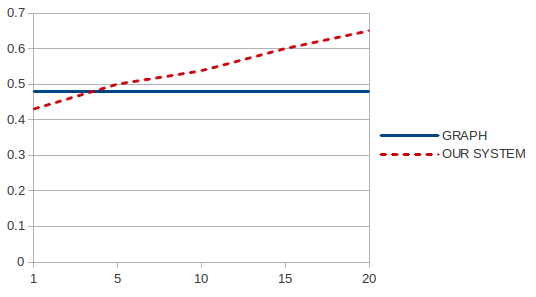
\includegraphics[width=\textwidth]{images/furniturePrec.png}
%\end{figure}
\end{minipage}
%\begin{figure}[ht]
\begin{minipage}{0.50\linewidth}
\centering
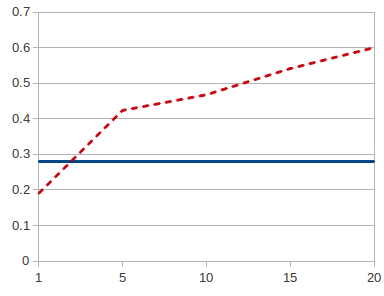
\includegraphics[width=\textwidth]{images/precP.png}
\end{minipage}
\caption{Comparison of the accuracy of the Graph algorithm and our system. The x axis shows indicates that the accuracy was calculated considering the x first REs in the ranking. The y axis indicates the accuracy. Our system is depicted as a dotted line and the Graph system as a continuous line.\label{graficoPresicion}}
\end{figure}

 

%The dotted line is that represented by our system and the another is that represents the GRAPH performance.

%Also we analyze the RE founded in the corpus that the system does not generate in a first frequency, and found that there were a 13.75\% in furniture that were not RE, those were underspecified sentences with does not identifies the target object. For people the proportion was lower just a 5.88\%. We saw that when a person used another word that was not taking into account in the annotation of the corpus, it was annotated as ``other'', and our system was not capable of generate ``other'' because it was not in the model.
%In the table~\ref{error-furniture} there is a percentage of times in 100 runs that the system does not generates the RE given by the human for furniture, and as showed in Table~\ref{error-people} the human were more difficult to generate in the first 100 because the RE were longer the RE have less probability of occur. If the system does not generates the RE in 100 of runs does not mean that the system could not generate them, it just mean that the system need to be running more in order to generate this RE.\\


%\begin{table}[h!]
%\begin{center}
%\begin{tabular}{|l|c|c|}
%\hline
%		& Count		& Percentage\\
%\hline
%It is not RE	&	11	&	13.75 \\
%%		&	37	&	46.25\% \\
%Contains ``other''	&	6	&	7.50 \\
%\hline
%SYS does not generated the RE in 100 runs	&	8	&	10.00 \\
%SYS generated but not with higher frequency	&	18	&	22.5 \\
%\hline
%\end{tabular}
%%\vspace*{.1cm}
%\caption{Clasification of RE that the system could not generates or generates with low frequency for Furniture}
%\label{error-people}
%\end{center}
%\end{table}
%%\vspace*{-.4cm}

%\begin{table}[h!]
%\begin{center}
%\begin{tabular}{|l|c|c|}
%\hline
%			& Count		& Percentage\\
%\hline
%It is not RE		&	4	&	5.88 \\
%Contains ``other''	&	6	&	8.82 \\
%\hline
%SYS does not generated the RE in 100 runs	&	17	&	25.00 \\
%SYS generated but not with higher frequency	&	28	&	41.18 \\
%%BIEN			&	13	&	19.12\% \\

%\hline
%\end{tabular}
%%\vspace*{.1cm}
%\caption{Clasification of RE that the system could not generates or generates with low frequency for People}
%\label{error-furniture}
%\end{center}
%\end{table}
%%\vspace*{-.4cm}

\subsection{Human evaluation} \label{sec:humanevaluation}

We asked two human judges native speakers of English to evaluate our referring expressions via an experiment on the web. The authors of the paper did not participate during the evaluation. The judges could register to the evaluation system so that they did not have to complete it in one go, the could come back to it later. During the evaluation we showed each judge the scenes and two randomly ordered REs. One RE corresponded to the RE present in the corpus and produced by a person and the other RE corresponded to the top 1 RE produced by our system. We asked the judges to select the RE that would be more useful to identify the target in the scene. That is, to select it from among the other objects in the stimulus pictures. 

Our goal is to show that even if the RE generated by our algorithm does not coincide with the RE produced by a human in the corpus collection, it can be judged as good or even better than the REs generated by humans. 

%\begin{table}[h!]
%\begin{center}
%\begin{tabular}{|c|c|c|c|}
%\hline
%           & Agree in & Not agree & Total\\
%\hline 
%Furniture & 25       & 18        & 43 \\
%People    & 25       & 30        & 55 \\
%Total     & 50       & 48        & 98 \\
%\hline
%\end{tabular}
%\caption{Agree between judges} 
%\label{agree-judges}
%\end{center}
%\end{table}

%esta tabla no ayuda...no se que decir, no se como justificar que no coincidan...
%In the Table~\ref{agree-judges} we can see that the both judges choice the same RE 25 times for Furniture and 25 times for People, 

\begin{table}[h!]
\begin{center}
\begin{tabular}{|l|c|c|c|c|}
\hline
%total scenes in evaluation set &                           80   &             68
 & Furniture domain & People domain & Weighted mean \\
\hline
system equal to human  	&	.46	&	.19	&	.33 \\
system better to human by 2 judges &	.29 	& 	.24 	& 	.27 \\
system better to human by 1 or 2 judges & .51	&	.68	&	.59 \\
system worse to human by 2 judges &	.03	&	.13	&	.08 \\
system equal or better to human by 2 judge  &.75  &       .43	&       .60 \\
system equal or better to human by 1 judge  &.97	&	.87	&	.92 \\
\hline
\end{tabular}
%\vspace*{.1cm}
\caption{Porcentage of system versus human selected choices} 
\label{system-versus-human}
\end{center}
\end{table}
%\vspace*{-.9cm}
In the Table~\ref{system-versus-human} we show the porcentage of the judges selections, the judge selected more the RE generated by our system than the human RE.

%\begin{table}[h!]
%\begin{center}
%\begin{tabular}{|c|c|c|c|}
%\hline
%Judge    & Human choice & System choice & Total\\
%\hline 
%Judge1 & 25       & 30        & 55 \\
%Judge2    & 23       & 32        & 55 \\
%\hline
%\end{tabular}
%\caption{System versus human selected choice for People} 
%\label{system-versus-human-people}
%\end{center}
%\end{table}

%In the case of pictures of people you can see in the Table~\ref{system-versus-human-people} that the judges selected more RE generated by our system but the diference in not very significant.

\begin{table}[h!]
\begin{center}
\begin{tabular}{|c|c|c|c|c|c|}
\hline
           & System & System (\%) & Human & Human (\%) & Total\\
\hline
Furniture & 23  & .92 &  2 & .08  & 25 \\
People    & 16  & .64 & 9  & .36 & 25 \\
\hline
Total     & 39  & .78    & 11 & .22 & 50  \\
\hline
\end{tabular}
%\vspace*{.1cm}
\caption{Coincidences between judges, the system is the prefered the 78\% of times} 
\label{system-better}
\end{center}
\end{table}
%\vspace*{-.9cm}
Taking into account just the coincidences between jugdes the Table~\ref{system-better} shows the percentage of their preference, they prefered the system in 78\% of times.

Sometimes comparison was unfair because human gives a RE that includes relation that were not annotated so, the system haven't the posibility of produce them. A point in favor of the system is that sometimes the human did an underespecified RE and the system has a better one.\\

In Figure~\ref{smallBlueFan1} the human RE was ``blue frontal chair'', and the system ``the blue bottom chair'' the judge selected the system RE, in this case our intuition is that the property ``bottom'' helps more than the property ``frontal'' which have a probability lower in our system. Another times just RE given by the system was intuitivelly less complex than the human one like in Figure~\ref{smallBlueFan} where RE of the system was ``small blue fan'' and the human RE was ``bottom row, blue fan''.
\begin{figure}[ht]
\begin{minipage}{0.50\linewidth}
\centering
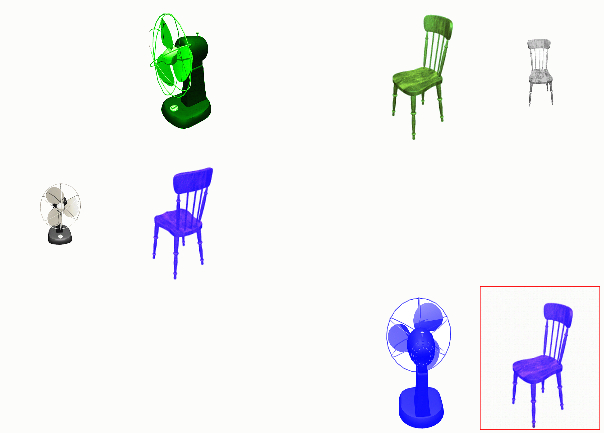
\includegraphics[width=\textwidth]{images/tuna.jpg} % esta es la 101t5 la que mostramos al principio
\caption{Scene used during the collection of the TUNA corpus. The human RE was ``blue frontal chair'', and the system ``the blue bottom chair''. Judges prefer the system generated.}
\label{smallBlueFan1}
\end{minipage}
\begin{minipage}{0.50\linewidth}
\centering
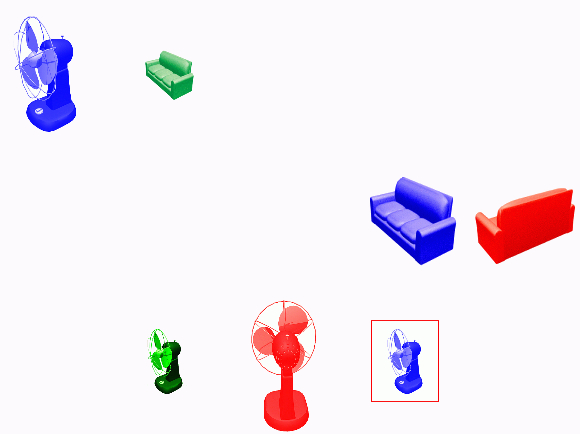
\includegraphics[width=\textwidth]{images/smallBlueFan.jpg}
\caption{Scene used during the collection of the TUNA corpus. The human RE ``bottom row, blue fan'', and the system ``small blue fan''. Judges prefer the system generated.}
\label{smallBlueFan}
\end{minipage}
\end{figure}

%Sometimes the judges choice the human RE for example in Figure~\ref{largeGreyChair} the
%system RE was ``large grey chair facing away'' and the human RE was ``the top left grey chair''.

%\begin{figure}[ht]
%%\begin{minipage}{0.50\linewidth}
%\centering
%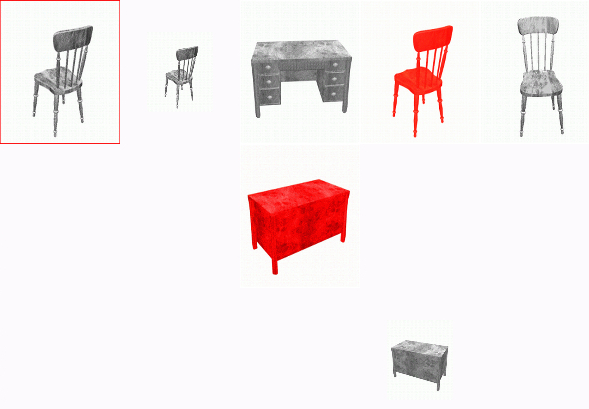
\includegraphics[width=0.8\textwidth]{images/largeGreyChair.jpg}
%\caption{TUNA corpus furniture scene}
%\label{largeGreyChair}
%\end{figure}

\begin{figure}[ht]
\begin{minipage}{0.50\linewidth}
\centering
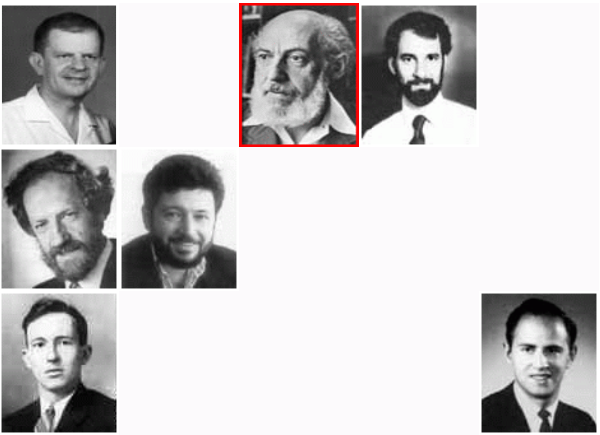
\includegraphics[width=\textwidth]{images/s28t25.png}
\caption{Scene used during the collection of the TUNA corpus. The human  RE was ``man on top row in middle'', and the system ``man in the middle column''. Judges prefer the human RE.}
\label{s28t25}
%\end{figure}
\end{minipage}
%\begin{figure}[ht]
\begin{minipage}{0.50\linewidth}
\centering
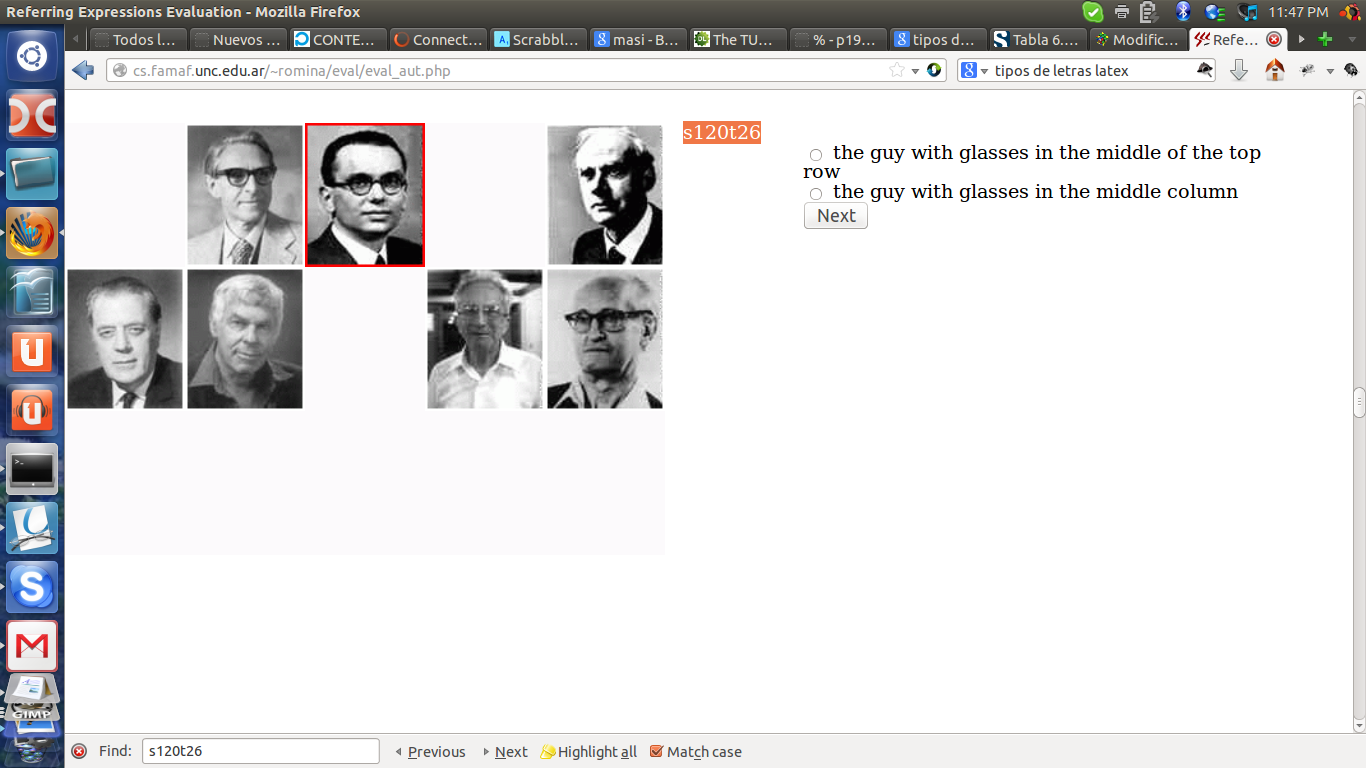
\includegraphics[width=\textwidth]{images/s120t26.png}
\caption{Scene used during the collection of the TUNA corpus. The human RE was ``the guy with glasses in the middle of the top row'', and the system ``the guy with glasses in the middle column''. Judges were not agree in their preference.}
\label{s307t21}
\end{minipage}
\end{figure}

There were cases in which the judges choice the human RE for example in Figure~\ref{s28t25}~the human RE was more overspecified with ``on top row'' than the system, here the human gives a RE that includes both axis in the grid and the system just one, this kind of RE were the person includes both axis information was a property that was not captured by our system.

In Figure~\ref{s307t21}~we show an example in which both judge were not agree and they select one the human RE and other the system RE.  The human RE was ``the guy with glasses in the middle of the top row'', and the system ``the guy with glasses in the middle column'', in this case we see that not always human prefer RE that includes both axis of the grid.

